\chapter{Design}
\label{chapter:Design}
%Overarching design in a top-down view: 
%-describe file system, 
%-server/client design overall architecture
%-how protocol is peformed by the server
%-describe current functionality of the implementation. Handles protocol run, view-changes and checkpointing

%old version:-overall usage over different parameters, overaching stuff thats not the actual implementation of the algorithm, but the network layer to server to algorithm, how to run the algorithm/checkpointing/view changes.
\begin{wrapfigure}{r}{0.45\linewidth}
\centering
%\vspace{15pt}
%\rule{0.9\linewidth}{0.75\linewidth}
% ,scale=0.8, every node/.style={scale=0.8}
\iffalse
\begin{wrapfigure}{r}{0.3\linewidth}
\centering
\vspace{15pt}
%\rule{0.9\linewidth}{0.75\linewidth}
% ,scale=0.8, every node/.style={scale=0.8}
\tikzstyle{every node}=[draw=black,thick,anchor=west]
    \begin{tikzpicture}[%
      grow via three points={one child at (0.5,-0.7) and
      two children at (0.5,-0.7) and (0.5,-1.4)},
      edge from parent path={(\tikzparentnode.south) |- (\tikzchildnode.west)}]
      \node {PBFT}
        child { node {App.cs}}
        child { node {Certificates}
          child { node {Protocol}}
          child { node {Reply}}
          child { node {ViewChange}}
          child { node {Checkpoint}}
        }
        child [missing] {}				
        child [missing] {}		
        child [missing] {}
        child [missing] {}		
        child { node {Messages}
          child { node {Session}}
          child { node {Request}}
          child { node {Phase}}
          child { node {Reply}}
          child { node {ViewChange}}
          child { node {NewView}}
          child { node {Checkpoint}}
        }
        child [missing] {}				
        child [missing] {}
        child [missing] {}
        child [missing] {}
        child [missing] {}
        child [missing] {}
        child [missing] {}
        child { node {Helper}
          child { node {Crypto}}
          child { node {Deserializer}}
          child { node {Serializer}}
          child { node {Enums}}
        }
        child [missing] {}
        child [missing] {}
        child [missing] {}
        child [missing] {}
        child { node {Replica}
          child { node {Server}}
          child { node {ProtocolExecution}}
        }
        child [missing] {}
        child [missing] {}
        child {node {Network}
          child { node {Listener}}
          child { node {Interactive Connection}}
        };
    \end{tikzpicture}
\fi

\tikzstyle{every node}=[draw=black,thick,anchor=west]
    \begin{tikzpicture}[%
      grow via three points={one child at (0.5,-0.7) and
      two children at (0.5,-0.7) and (0.5,-1.4)},
      edge from parent path={(\tikzparentnode.south) |- (\tikzchildnode.west)}]
      \node {PBFT}
        child { node {App.cs}}
        child { node {Certificates}
        	child {node {...}}
        	}	
        child [missing] {}
        child { node {Messages}
        	child {node {...}}
        	}
        child [missing] {}
        child { node {Helper}
        	child {node {...}}
        	}
        child [missing] {}
        child { node {Replica}
          child { node {Server.cs}}
          child { node {Network}
          	child {node {...}}
        	}
        child [missing] {}
          child { node {Protocol}
          child {node {...}}
        	}
        };
    \end{tikzpicture}
    \caption{Summary of the file architecture for the PBFT implementation}
    \label{fig:filestruct}
    \vspace{40pt}
\end{wrapfigure}

\begin{figure}[]
	\centering
	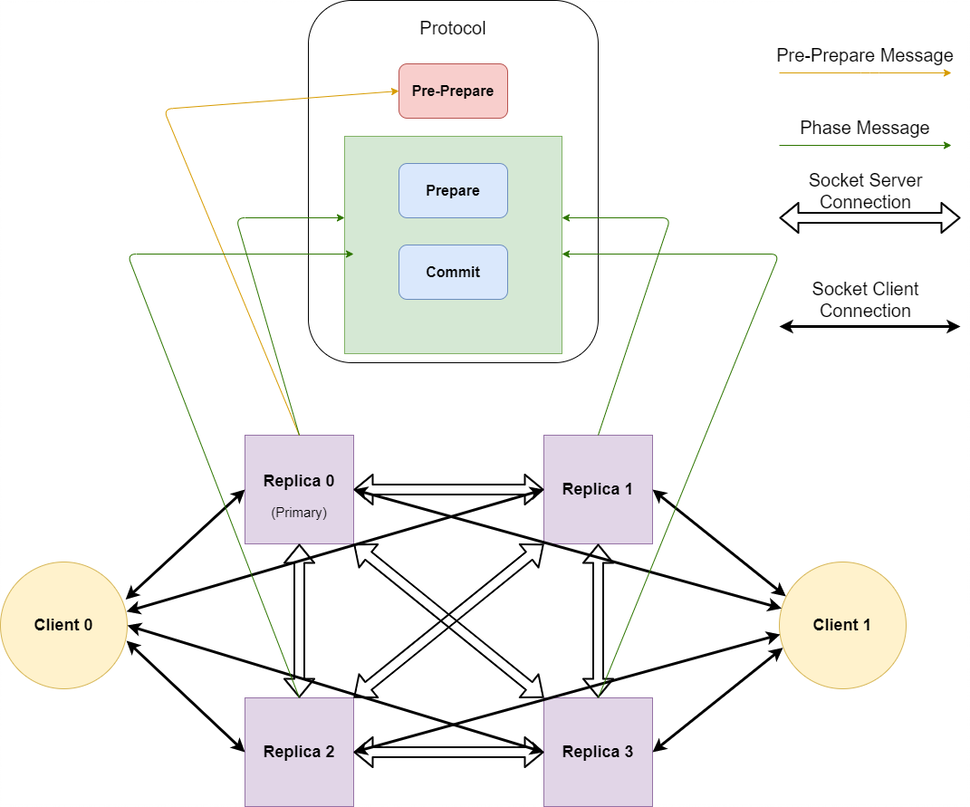
\includegraphics[width=\linewidth]{figures/meshnetwork}
	\caption{Overall architecture of the PBFT implementation networking}
	\label{fig:meshnetwork}
\end{figure}